\subsection{Experimental Results}
\label{subsec:performanceComparison_results}

%---------------------- ACO VS SSO ---------------------

Table \vref{table:performanceComparison_ACOSSOBEST} shows the average produced results, concerning the performance criteria, of the proposed algorithm and the plain ACO implementation. Representation of the best route set, having for routes, produced by SSO is seen in Table \vref{table:performanceComparison_bestRouteSet4}.  Representation of the best route set, having for routes, produced by ACO is found in \vref{table:performanceComparison_bestRouteSet4_ACO}. Best, worst, average, and median produced results in addition to the STD is presented in Table \vref{table:performanceComparison_ACOFull}.

    \begin{table}[H]
    \centering
    \begin{tabular}{|l||l|l|l|l|l|}
    \hline
    Algorithm & $d_0(\%)$ & $d_1(\%)$ & $d_2(\%)$ & $d_{unsat}(\%)$ & $ATT$ \\
    \hline
    ACO Average & 81.92 & 16.13 & 1.86 & 0.09 & 10.43\\
    \hline
    SSO Average & 85.21 & 13.49 & 1.30 & 0.00 & 10.27\\
    \hline
    \end{tabular}
    \caption {Comparing the best route set of a plain ACO implementation (ACO) and the proposed algorithm (SSO), having four routes.}
    % 50 runs
    \label{table:performanceComparison_ACOSSOBEST}
    \end{table}

   

%-------------------- 4 route sets ---------------------

%Best Ants Route: {[14,13,11,10,8,6,15,7,][1,2,3,6,8,10,11,12,][14,10,8,6,4,5,2,3,][9,15,7,10,11,12,4,2,]}
\begin{table}[H]
    \centering
    \begin{tabular}{|l|llllllll|}
    \hline
    Route 1: & 14 & 13 & 11 & 10 & 8 & 6 & 15 & 7 \\
    Route 2: & 1 & 2 & 3 & 6 & 8 & 10 & 11 & 12 \\
    Route 3: & 14 & 10 & 8 & 6 & 4 & 5 & 2 & 3 \\
    Route 4: & 9 & 15 & 7 & 10 & 11 & 12 & 4 & 2 \\
	\hline
    \end{tabular}
    \caption {Representation of the best route set, having four routes, constructed by the proposed algorithm.}
    \label{table:performanceComparison_bestRouteSet4}
\end{table}

\begin{figure}[H]
    \begin{center}
    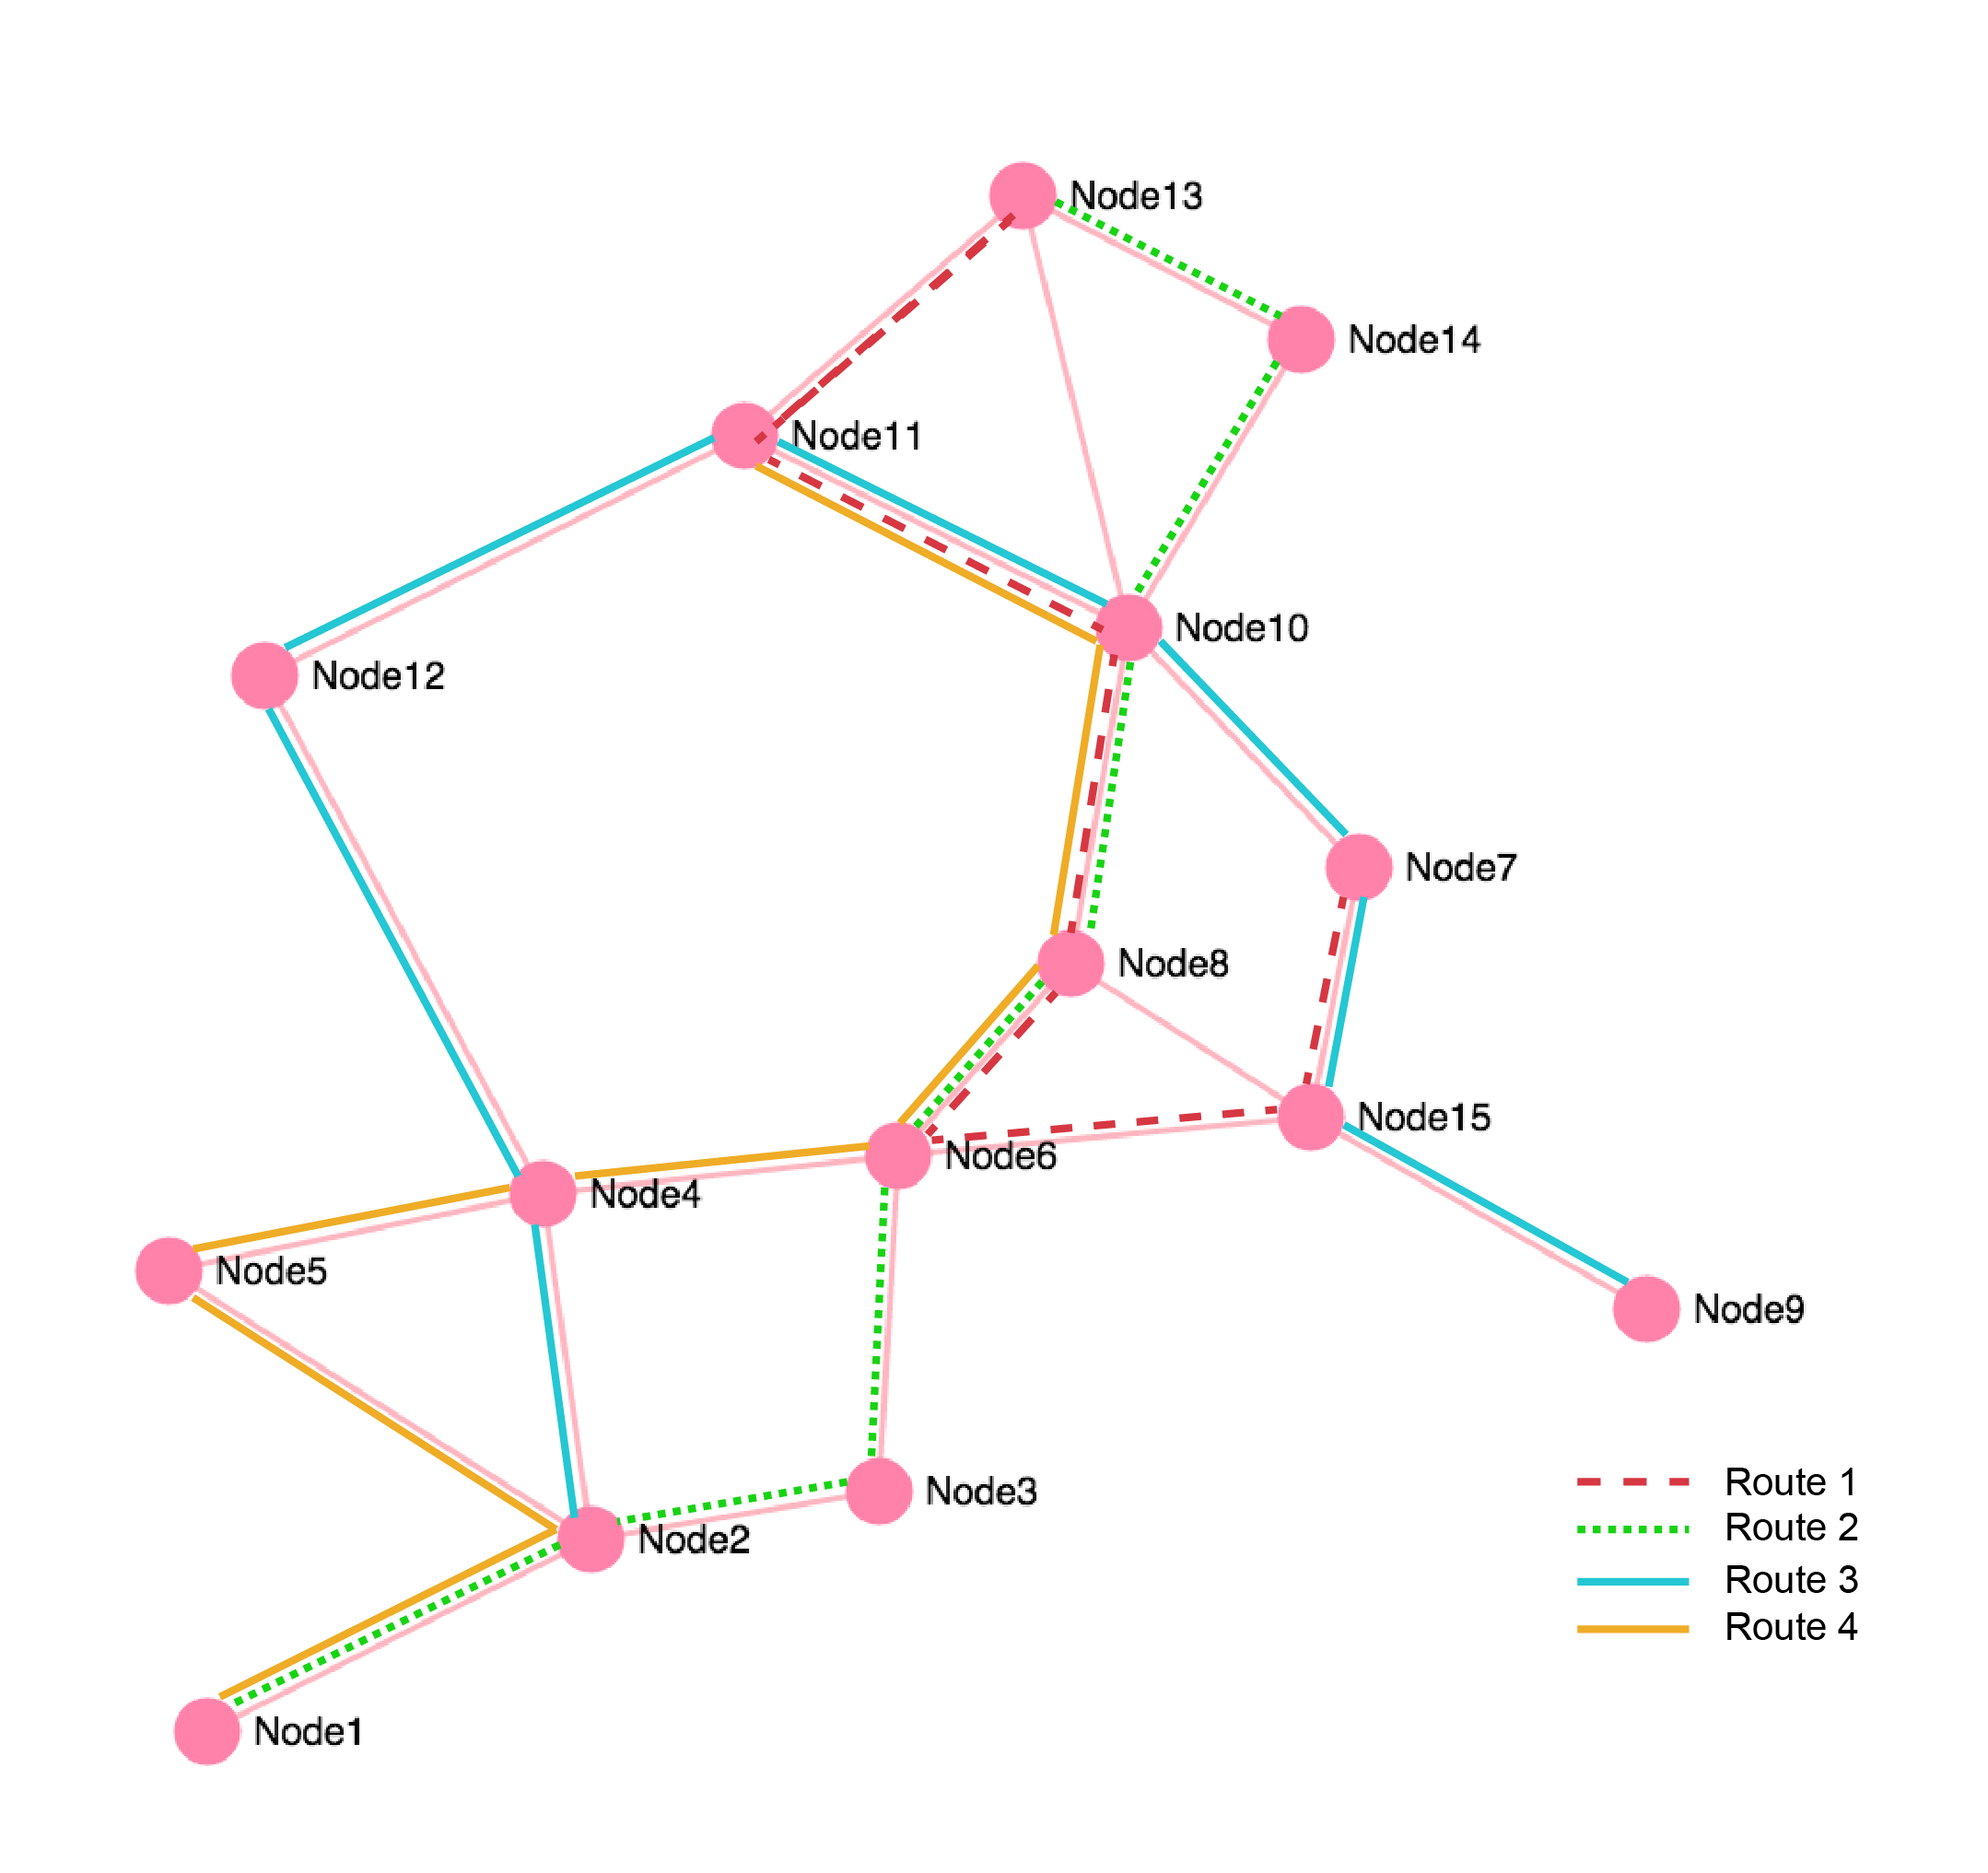
\includegraphics[width=4in]{assets/mandlnetwork_4routes.png}
    \end{center}
    \caption{Illustration of the best route set, having four routes, constructed by the proposed algorithm (Mandl's transit network as a graph)}
    \label{fig:bestRouteSet4} 
\end{figure}

Table \vref{table:performanceComparison_4} presents the results produced by the proposed algorithm (SSO), having four routes, and results from route sets constructed by other approaches.

\begin{table}[H]
	\centering
    \hspace*{-1.0cm}
    \begin{tabular}{|l||l|l|l|l|l|}
 	\hline
 	Algorithm & $d_0(\%)$ & $d_1(\%)$ & $d_2(\%)$ & $d_{unsat}(\%)$ & $ATT$ \\
 	\hline
    \citet{mandl79} & 69.94 & 29.93 & 0.13 & 0.00 & 12.90 \\
    \citet{kechagiopoulos14} avg & 90.52 & 8.75 & 0.73 & 0.00 & 10.71 \\
    \citet{kechagiopoulos14} best & 91.84 & 7.64 & 0.51 & 0.00 & 10.64 \\
    \citet{nikolic14} avg & 95.05 & 4.95 & 0.00 & 0.00 & -$^b$ \\
    \citet{kidwai98} & 72.95 & 26.91 & 0.13 & 0.00 & 12.72 \\
    \citet{fan10} best & 93.26 & 6.74 & 0.00 & 0.00 & 11.37 \\
    \citet{fan10} HC avg & 91.83 & 8.17 & 0.00 & 0.00 & 11.69 \\
    \citet{fan10} SA avg & 92.48 & 7.52 & 0.00 & 0.00 & 11.55 \\
    \citet{chakroborty02} & 86.86 & 12.00 & 1.14 & 0.00 & 11.90 \\
    \citet{zhang10} & 91.46 & 8.54 & 0.00 & 0.00 & 10.65 \\
    \citet{chew12} avg & 92.88 & 6.91 & 0.20 & 0.00 & 11.16 \\
    \citet{chew12} best & 93.71 & 6.29 & 0.00 & 0.00 & 10.82 \\
	\hline
    \hline
    SSO Best & 87.73 & 10.98 & 1.28 & 0.00 & 10.03\\
    SSO Average & 85.21 & 13.49 & 1.30 & 0.00 & 10.27\\
    SSO Median & 85.81 & 13.29 & 1.09 & 0.00 & 10.26\\
    SSO Worst & 76.56 & 22.16 & 1.28 & 0.00 & 10.01\\
    SSO Standard Deviation & 2.66 & 2.70 & 0.84 & - & 0.18\\
    %SSO Confidence interval$^b$ & ~ & ~ & ~ & ~ & ~ \\
    \hline
    \end{tabular}
    \caption {Comparing the best route set, having four routes, produced by the proposed algorithm(SSO) with route sets constructed by other approaches.}
    \begin{itemize}[noitemsep]
    %\item[$^a$:] mintues per user
    \item[$^b$:] 
    %\item[$^b$:] Confidence Interval with a confidence level of 95\%
    \end{itemize}
    \label{table:performanceComparison_4}
\end{table}


%-------------------- 6 route sets ---------------------
%Best Ants Route: {[12,11,10,13,14,][9,15,7,10,14,13,11,12,][7,10,8,6,4,5,2,3,][1,2,3,6,8,10,11,13,][1,2,4,6,3,][14,13,10,7,15,6,4,12,]}
    \begin{table}[H]
    \centering
    \begin{tabular}{|l|l l l l l l l l|}
    \hline
    Route 1: & 12 & 11 & 10 & 13 & 14 &  &  &  \\
    Route 2: & 9 & 15 & 7 & 10 & 14 & 13 & 11 & 12 \\
    Route 3: & 7 & 10 & 8 & 6 & 4 & 5 & 2 & 3 \\
    Route 4: & 1 & 2 & 3 & 6 & 8 & 10 & 11 & 13 \\
    Route 5: & 1 & 2 & 4 & 6 & 3 &  &  &  \\
    Route 6: & 14 & 13 & 10 & 7 & 15 & 6 & 4 & 12 \\
    \hline
    \end{tabular}
    \caption {The best route set, having six routes}
    \label{table:performanceComparison_bestRouteSet6}
    \end{table}


    \begin{figure}[H]
    \begin{center}
    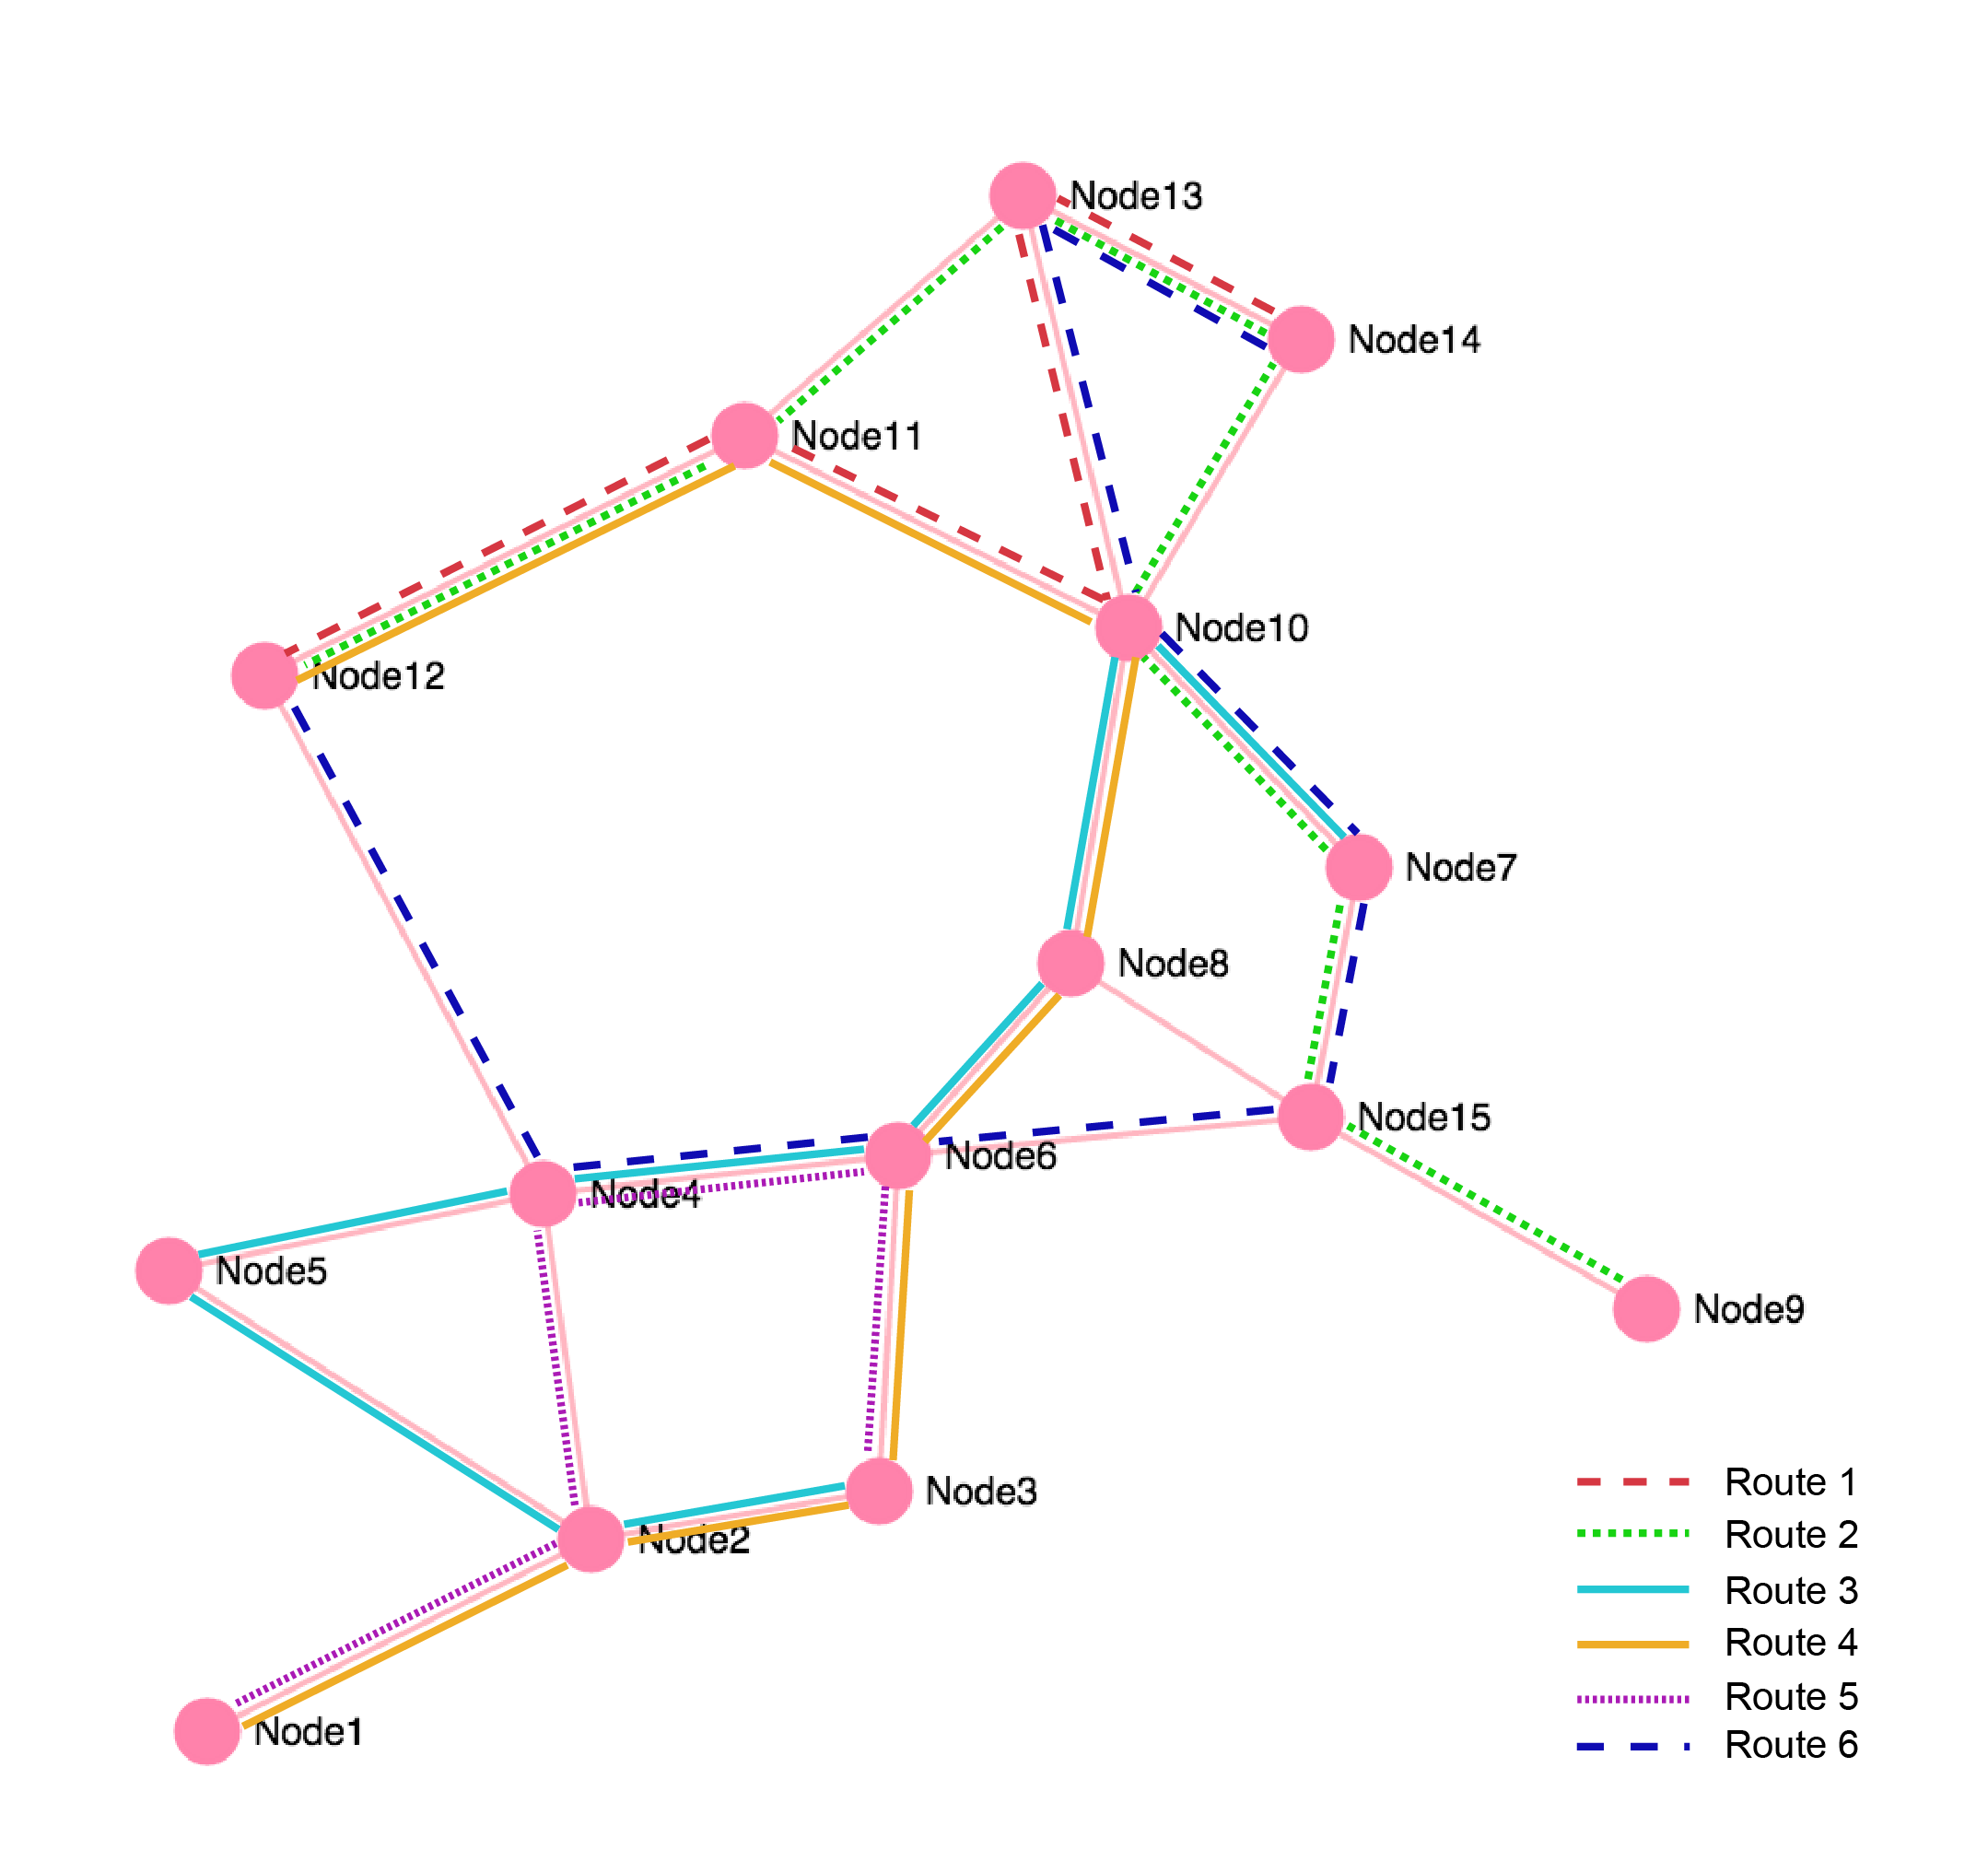
\includegraphics[width=4in]{assets/mandlnetwork_6routes.png}
    \end{center}
    \caption{Illustration of the best route set, having six routes, constructed by the proposed algorithm (Mandl's transit network as a graph)}
    \label{fig:bestRouteSet6} 
\end{figure}

    \begin{table}[H]
    \centering
    \hspace*{-1.0cm}
    \begin{tabular}{|l||l|l|l|l|l|}
    \hline
    Algorithm & $d_0(\%)$ & $d_1(\%)$ & $d_2(\%)$ & $d_{unsat}(\%)$ & $ATT$ \\
    \hline
    \citet{kechagiopoulos14} avg & 95.62 & 4.28 & 0.10 & 0.00 & 10.28 \\
    \citet{kechagiopoulos14} best & 96.21 & 3.47 & 0.32 & 0.00 & 10.23 \\
    \citet{nikolic14} & 94.34 & 5.65 & 0.00 & 0.00 & - \\
    \citet{kidwai98} & 77.92 & 19.62 & 2.40 & 0.00 & 10.78 \\
    \citet{fan10} best & 91.52 & 8.48 & 0.00 & 0.00 & 10.48  \\
    \citet{fan10} HA avg & 90.23 & 9.26 & 0.51 & 0.00 & 11.69 \\
    \citet{fan10} SA avg & 90.87 & 8.74 & 0.39 & 0.00 & 10.65 \\
    \citet{chakroborty02} & 86.04 & 13.96 & 0.00 & 0.00 & 10.30 \\
    \citet{zhang10} & 91.12 & 8.88 & 0.00 & 0.00 & 10.50 \\
    \citet{chew12} avg & 93.85 & 5.88 & 0.24 & 0.03 & 10.51 \\
    \citet{chew12} best & 95.57 & 4.43 & 0.00 & 0.00 & 10.28 \\
    \citet{baaj91} & 78.61 & 21.39 & 0.00 & 0.00 & 11.86 \\
    \hline
    \hline
    SSO Best & 89.53 & 9.25 & 1.22 & 0.00 & 10.03\\
    SSO Average & 87.17 & 12.0 & 0.82 & 0.01 & 10.11\\
    SSO Median & 87.93 & 10.98 & 0.77 & 0.00 & 10.03\\
    SSO Worst & 82.47 & 17.41 & 0.13 & 0.00 & 10.03\\
    SSO Standard Deviation & 2.74 & 2.78 & 0.63 & 0.02 & 0.14\\
    \hline
    \end{tabular}
    \caption {Comparing the best route set, having six routes, produced by the proposed algorithm with route sets constructed by other approaches.}
    \label{table:performanceComparison_6}
    \end{table}

%-------------------- 7 route sets ---------------------
%Best Ants Route: {[12,11,10,8,6,4,5,2,][9,15,7,10,14,13,11,12,][11,12,4,5,2,3,6,8,][12,11,10,8,6,3,2,4,][4,6,15,7,10,13,14,][13,10,14,][1,2,3,6,8,10,14,13,]}

\begin{table}[H]
    \centering
    \begin{tabular}{|l|l l l l l l l l|}
    \hline
    Route 1: & ~ & ~ & ~ & ~ & ~ & ~ & ~ & ~ \\
    Route 2: & ~ & ~ & ~ & ~ & ~ & ~ & ~ & ~ \\
    Route 3: & ~ & ~ & ~ & ~ & ~ & ~ & ~ & ~ \\
    Route 4: & ~ & ~ & ~ & ~ & ~ & ~ & ~ & ~ \\
    Route 5: & ~ & ~ & ~ & ~ & ~ & ~ & ~ & ~ \\
    Route 6: & ~ & ~ & ~ & ~ & ~ & ~ & ~ & ~ \\
    Route 7: & ~ & ~ & ~ & ~ & ~ & ~ & ~ & ~ \\
    \hline
    \end{tabular}
    \caption {The best route set, having seven routes \emph{\color{blue} TODO:}}
    \label{table:performanceComparison_bestRouteSet7}
    \end{table}

    \begin{table}[H]
    \centering
    %\hspace*{-2.0cm}
    \begin{tabular}{|l||l|l|l|l|l|}
    \hline
    Algorithm & $d_0(\%)$ & $d_1(\%)$ & $d_2(\%)$ & $d_{unsat}(\%)$ & $ATT$ \\
    \hline
    \citet{kechagiopoulos14} avg & 96.55 & 3.45 & 0.01 & 0.00 & 10.23 \\
    \citet{kechagiopoulos14} best & 97.17 & 2.83 & 0.00 & 0.00 & 10.16 \\
    \citet{nikolic14} & 94.41 & 5.59 & 0.00 & 0.00 & - \\
    \citet{kidwai98} & 93.91 & 6.09 & 0.00 & 0.00 & 10.70 \\
    \citet{fan10} best & 93.32 & 7.13 & 0.32 & 0.00 & 10.42  \\
    \citet{fan10} HC avg & 92.21 & 7.13 & 0.66 & 0.00 & 10.74 \\
    \citet{fan10} SA avg & 92.47 & 6.95 & 0.58 & 0.00 & 10.62 \\
    \citet{chakroborty02} & 89.15 & 10.85 & 0.00 & 0.00 & 10.15 \\
    \citet{zhang10} & 92.89 & 7.11 & 0.00 & 0.00 & 10.46 \\
    \citet{chew12} avg & 96.47 & 3.53 & 0.00 & 0.00 & 10.31 \\
    \citet{chew12} best & 95.57 & 4.42 & 0.00 & 0.00 & 10.27 \\
    \citet{baaj91} & 80.99 & 19.01 & 0.00 & 0.00 & 12.50 \\
    \hline
    \hline
    SSO Best & 89.85 & 8.67 & 1.48 & 0.0 & 10.03\\
    SSO Average & 88.49 & 10.72 & 0.79 & 0.0 & 10.08\\
    SSO Median & 88.12 & 10.92 & 0.9 & 0.0 & 10.03\\
    SSO Worst & 83.94 & 15.93 & 0.13 & 0.0 & 10.01\\
    SSO Standard Deviation & 2.29 & 2.32 & 0.42 & 0.02 & 0.08\\
    \hline
    \end{tabular}
    \caption {Comparing the best route set, having seven routes, produced by the proposed algorithm with route sets constructed by other approaches.}
    \label{table:performanceComparison_7}
    \end{table}
%-------------------- 8 route sets ---------------------
%Best Ants Route: {[11,10,8,6,3,2,1,][13,14,10,7,15,9,][5,4,12,11,10,7,15,6,][11,10,8,6,3,2,5,4,][10,7,15,6,3,2,4,5,][9,15,7,10,11,13,14,][13,14,10,8,6,4,5,2,][5,4,2,3,6,8,15,7,]}
\begin{table}[H]
    \centering
    \begin{tabular}{|l|l l l l l l l l|}
    \hline
    Route 1: & ~ & ~ & ~ & ~ & ~ & ~ & ~ & ~ \\
    Route 2: & ~ & ~ & ~ & ~ & ~ & ~ & ~ & ~ \\
    Route 3: & ~ & ~ & ~ & ~ & ~ & ~ & ~ & ~ \\
    Route 4: & ~ & ~ & ~ & ~ & ~ & ~ & ~ & ~ \\
    Route 5: & ~ & ~ & ~ & ~ & ~ & ~ & ~ & ~ \\
    Route 6: & ~ & ~ & ~ & ~ & ~ & ~ & ~ & ~ \\
    Route 7: & ~ & ~ & ~ & ~ & ~ & ~ & ~ & ~ \\
    Route 8: & ~ & ~ & ~ & ~ & ~ & ~ & ~ & ~ \\
    \hline
    \end{tabular}
    \caption {The best route set, having eight routes \emph{\color{blue} TODO:}}
    \label{table:performanceComparison_bestRouteSet8}
    \end{table}

    \begin{table}[H]
    \centering
    \hspace*{-1.0cm}
    \begin{tabular}{|l||l|l|l|l|l|}
    \hline
    Algorithm & $d_0(\%)$ & $d_1(\%)$ & $d_2(\%)$ & $d_{unsat}(\%)$ & $ATT$ \\
    \hline
    \citet{kechagiopoulos14} avg & 97.47 & 2.53 & 0.00 & 0.00 & 10.17 \\
    \citet{kechagiopoulos14} best & 97.75 & 2.25 & 0.00 & 0.00 & 10.13 \\
    \citet{nikolic14} & 96.40 & 3.60 & 0.00 & 0.00 & - \\
    \citet{kidwai98} & 84.73 & 15.27 & 0.00 & 0.00 & 12.22 \\
    \citet{fan10} best & 94.54 & 5.46 & 0.00 & 0.00 & 10.36 \\
    \citet{fan10} Hill Climbing & 93.23 & 6.18 & 0.59 & 0.00 & 10.69 \\
    \citet{fan10} Simulated Annealing & 93.65 & 5.88 & 0.47 & 0.00 & 10.58 \\
    \citet{chakroborty02} & 90.38 & 9.58 & 0.00 & 0.00 & 10.46 \\
    \citet{zhang10} & 93.14 & 6.86 & 0.00 & 0.00 & 10.42 \\
    \citet{chew12} avg & 96.16 & 3.84 & 0.00 & 0.09 & 10.31 \\
    \citet{chew12} best & 97.82 & 2.18 & 0.00 & 0.09 & 10.19 \\
    \citet{baaj91} & 79.96 & 20.04 & 0.00 & 0.00 & 11.86 \\
    \hline
    \hline
    SSO Best & 91.01 & 7.9 & 1.09 & 0.0 & 10.01\\
    SSO Average & 89.16 & 10.05 & 0.8 & 0.0 & 10.06\\
    SSO Median & 88.7 & 10.21 & 0.77 & 0.0 & 10.03\\
    SSO Worst & 92.42 & 6.81 & 0.77 & 0.0 & 10.08\\
    SSO Standard Deviation & 2.24 & 2.14 & 0.68 & 0.0 & 0.07\\
    \hline
    \end{tabular}
    \caption {Comparing the best route set, having eight routes, produced by the proposed algorithm with route sets constructed by other approaches.}
    \label{table:performanceComparison_8}
    \end{table}

    %---------------------- Execution time ---------------------

\begin{table}[H]
    \centering
    \hspace*{-1.0cm}
    \begin{tabular}{|c|c|}
        \hline
        \textbf{Instance} & \textbf{Run Time$^1$ (secs)}\\
        \hline
        Mandl (4 routes) & 673.0\\
        \hline
        Mandl (6 routes) & 2442.1\\
        \hline
        Mandl (7 routes) & 3891.1\\
        \hline
        Mandl (8 routes) & 8515.9\\
        \hline
    \end{tabular}
    \caption{Average Runtime of 50 Runs for Experiments Using the Mandl Network}
    \begin{itemize}[noitemsep]
    \item[$^1$:] $s$ = 50, $i$ = 125)
    \end{itemize} 
    \label{tabel:runTimeMandl}
\end{table}

%Table \vref{table:performanceComparison_runtime} shows the average runtime for each run with 50 runs.

